\documentclass[border=10pt]{standalone}
\usepackage{pgfplots}
\usepgfplotslibrary{colorbrewer}
\usetikzlibrary{arrows.meta}
\pgfplotsset{compat=1.18}

\begin{document}
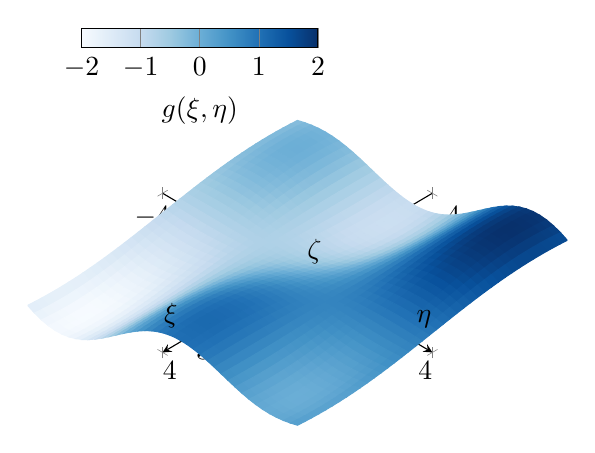
\begin{tikzpicture}
    \begin{axis}[
        title={},
        xlabel={$\xi$},
        ylabel={$\eta$},
        zlabel={$\zeta$},
        xmin=-4, xmax=4,
        ymin=-4, ymax=4,
        zmin=-4, zmax=2,
        view={135}{60},
        axis lines=center,
        axis line style={-stealth},
        xtick={-4,-3,...,4},
        ytick={-4,-3,...,4},
        ztick={-4,-3,...,2},
        grid=major,
        colormap/Blues,
        colorbar horizontal,
        colorbar style={
            at={(0.1,1.05)},
            anchor=south west,
            height=0.25cm,
            width=3cm,
            xlabel={$g(\xi, \eta)$},
            xtick={-2,-1,0,1,2},
        },
        ]
        \addplot3[
            surf,
            domain=-4:4,
            samples=40,
            faceted color=black,
            shader=flat,
        ]
        {sin(deg(x/2)) * cos(deg(y)) + sin(deg(y/2))};
    \end{axis}
\end{tikzpicture}
\end{document}